\documentclass{article}
\usepackage{amssymb}
\usepackage{amsmath}
\usepackage{amsbsy} % for bold greek
\usepackage{graphicx}
\usepackage{color}
\newcommand{\vect}[1]{\mathbf{#1}}
\renewcommand{\r}{\vect r}
\newcommand{\p}{\vect p}
\newcommand{\trmd}{\textrm{d}}
\renewcommand{\k}{\vect k}
\newcommand{\vnu}{\boldsymbol\nu}
\author{martin kielhorn}
\title{imaging through multimode fibers}
\date{summer 2014}
\begin{document}
\maketitle

\section{Einfaches Modell zur Propagation durch eine gest\"orte Faser}
Ich versuche mit mehreren einfachen Modellen zu verstehen, wie Licht
durch eine gekr\"ummte Faser propagiert. Zun\"achst betrachte ich als
einfachsten Fall eine Faser mit einem Knick (siehe Bild
\ref{fig:model}).
\begin{figure}[htbp]
  \centering
  \input{model.pdf_tex}
  \caption{model}
  \label{fig:model}
\end{figure}

Das eingestrahlte $E_\textrm{in}$ sei durch eine Superposition von
gef\"uhrten Moden $\phi_i$ der Faser ausgedr\"uckt.

\begin{align}
  E_\textrm{in} = \sum_i A_i \phi_i
\end{align}

F\"ur die weitere Diskussion sei ${\bf
  E_\textrm{in}}=(A_0,A_1,\ldots)$ der Vektor mit den komplexwertigen
Amplituden der einzelnen Fasermoden. Die Propagation durch ein gerades
Faserst\"uck der L\"ange $L$ erfolgt durch Multiplikation mit einen
Phasenfaktor $e^{i\beta_i L}$ f\"ur jede Mode. Hierbei ist $\beta_i$
die jeweils zur $i-$ten Mode geh\"orige Ausbreitungskonstante. Damit
l\"a\ss t sich die Propagation der Modenverteilung ${\bf
  E_\textrm{in}}$ durch eine Multiplikation mit der positiv definiten
Diagonalmatrix $P_L$ ausdr\"ucken:

\begin{align}
  P_L =
 \begin{pmatrix}
  e^{i\beta_0 L } & 0 & 0 & \cdots  \\
  0 & e^{i\beta_1 L } & 0 & \cdots  \\
  0 & 0 & e^{i\beta_2 L } & \cdots  \\
  \vdots  & \vdots  &  & \ddots &   \\
 \end{pmatrix}
\end{align}

Der Knick mit Winkel $\theta$ kann auch durch eine lineare Operation
auf den Modenverteilungen ausgedr\"uckt werden. Damit gilt f\"ur das
Feld hinter dem Knick:
\begin{align}
  {\bf E_\textrm{half}} = T_\theta P_{L_1} {\bf E_\textrm{in}} 
\end{align}
Wobei die Matrix $T_\theta$ die Kopplung der Moden am Knick
beschreibt.

F\"ur kleinen Knickwinkel $\theta \ll \lambda/a$ ergibt sich jede
Komponente $T_{\theta,\mu\nu}$ aus dem Integral \"uber ein Produkt aus
vier Termen \"uber den Faserquerschnitt ([1988Hill]). Der normierten
Feldverteilung der beiden Moden $\mu$ und $\nu$; dem Skalarprodukt
${\bf e_\mu\cdot e_\nu}$ der Einheitsfeldvektoren, die die
Polarisationsrichtung angeben und einem linearen Phasenfaktor
$e^{ik_\textrm{co}\theta x}$. Da beide Moden $\mu$ und $\nu$
symmetrisch in den Gleichungen vorkommen, ist auch die Kopplungsmatrix
symmetrisch:
\begin{align}
  T_\theta=T_\theta^T  
\end{align}


F\"ur den Spezialfall von schwach f\"uhrenden Wellenleitern mit
kreisf\"ormigen Querschnitt gibt [Marcuse1973] einen analytischen
Ausdruck des Modenkopplungsintegrals an. In diesem Fall koppeln
aufgrund der Rotationssymmetrie nur Moden mit gleicher azimuthaler
Quantenzahl ($l$) aber beliebiger radialer Quantenzahl $m$:
$\mu=\nu\pm m$. Das heisst, viele Entr\"age der Matrix $T_\theta$
verschwinden.

Damit kann das auf den Spiegel fallende Feld ausgedr\"uckt werden als:
\begin{align}
  {\bf E_\textrm{mirror}}= \underbrace{P_{L_2} T_\theta P_{L_1}}_M {\bf E_\textrm{in}} 
\end{align}
wobei ich mit $M$ die Transfermatrix vom Fasereingang zum
Faseraustritt bezeichne.

Der Spiegel bewirkt einen modenunabh\"angigen Phasensprung und koppelt
alle einlaufenden Moden in r\"ucklaufende Moden. Die zugeh\"orige
lineare Operation wird durch die Matrix 
\begin{align}
  R&=e^{i\pi}
  \begin{pmatrix}
    1 & 0 & \cdots  \\
  0 & 1 & \cdots  \\
  \vdots            &  & \ddots &   \\
 \end{pmatrix}
\end{align}
beschrieben.

Damit kann die Modenverteilung ${\bf E_\textrm{out}}$, die auf der
Fasereintrittseite wieder austritt beschrieben werden durch:

\begin{align}
  {\bf E_\textrm{out}} &=  \underbrace{P_{L_1} T_\theta P_{L_2}}_{M'} R  \underbrace{P_{L_2} T_\theta P_{L_1}}_M  {\bf E_\textrm{in}}
\end{align}
Ein interessantes Zwischenergebnis ist, dass $M'=M^T$. Dies
folgt aus der Symmetrie von $P_L$, $T_\theta$ und $R$ und dem Satz
$(AB)^T=B^TA^T$.

F\"ur mein Problem der Endoskopbildgebung ist eine wichtige Frage, ob
man aus einer Messung von $M^TRM$ auf $M$ schlie\ss en kann. Diese
Frage kann ich zur Zeit noch nicht beantworten.

Dieses Modell mit einem planaren Knick hat drei freie Parameter:
$L_1$, $L_2$ und $\theta$. Wenn die Transmissionsfunktion von
mindestens drei Fasermoden bekannt ist, k\"onnen diese Parameter
bestimmt werden. Hierbei ist jedoch zu bedenken, dass meine
holographische Vermessung der Faser die Phasen der Felder nur modulo
$2\pi$ bestimmt. Weiterhin setze ich zur Zeit kein ``common path''
Interferometer ein, so dass die absolute Phase zwischen den Messungen
driften kann. Ausserdem bin ich mir noch nicht sicher wie ich die
Modenverteilungen der Faser hinreichend genau bestimmen (numerisch
oder durch Kalibrierung) kann. Insbesondere ist unklar welche Moden
bei verschiedenen Winkeleinstellungen des fast steering mirrors
gestartet werden.

Alle diese technischen Probleme sollten sich jedoch l\"osen lassen,
zum Beispiel durch Verwendung mehrerer Laserwellenl\"angen und/oder
einem SLM basierten Aufbau wie in [2011Dholakia].

In Bild \ref{fig:model3} zeige ich wie das Modell des einzelnen Knicks
auf beliebig gebogene Fasern verallgemeinert werden kann durch viele
equidistant verteilte Knicke. Im allgemeinen Fall m\"ussen an jedem
Knick zwei Winkel bestimmt werden. Die Form der Faser kann umso besser
abgetastet werden, je mehr Moden vermessen werden k\"onnen.


\begin{figure}[htbp]
  \centering
  \input{model3.pdf_tex}
  \caption{model3}
  \label{fig:model3}
\end{figure}

Es w\"are interessant, einen Algorithmus zu entwickeln, der aus $M$
auf die $\theta_i$ schliesst. In diesem Zusammenhang k\"onnte man auch
analysieren wie lang eine Faser mit 10000 Moden sein kann, damit alle
$\theta_i$ bestimmt werden k\"onnen.

In einem n\"achsten Schritt w\"are zu untersuchen, ob man eine
kalibrierte Faser (mit bekannten $\theta_i$) die nur leicht verschoben
wird durch die Messung von nur wenigen Moden die Winkel $\theta_i$
rekalibrieren kann.

\section{multimode faser imaging im jones kalkuel}

% inkscape --export-latex -A setup.pdf setup.svg
\begin{figure}[htbp]
  \centering
  \input{setup.pdf_tex}
  \caption{setup}
  \label{fig:setup}
\end{figure}



\begin{figure}[htbp]
  \centering
  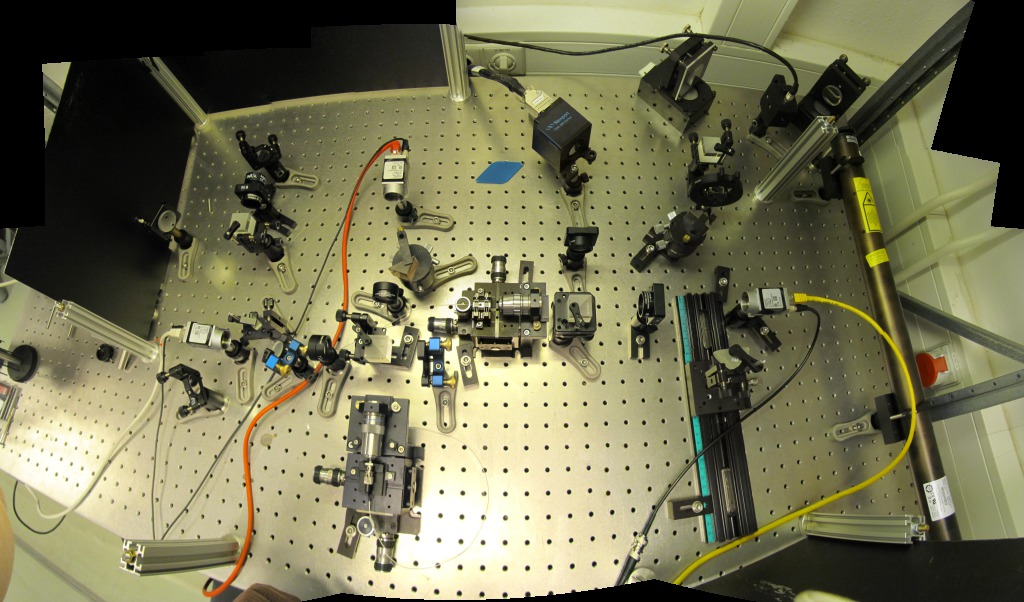
\includegraphics[width=12cm]{../multi-mode-imaging.jpg}
  \caption{Fotografie des Setups. }
  \label{fig:e40}
\end{figure}


\begin{figure}[htbp]
  \centering
  \includegraphics[width=12cm]{e40l.jpg}
  \caption{Fiber exit on the two cameras, illuminated by an LED.}
  \label{fig:e40}
\end{figure}

\begin{figure}[htbp]
  \centering
  \includegraphics[width=12cm]{e66led.jpg}
  \caption{Fiber entrance illuminated by LED. The indicated area
    depicts the region of interest containing the core of the fiber.}
  \label{fig:e66}
\end{figure}

\begin{figure}[htbp]
  \centering
  \includegraphics[width=7cm]{sm1.png}
  \includegraphics[width=7cm]{sm2.png}
  \includegraphics[width=7cm]{sm3.png}
  \caption{abs2 of the fields of the 3 cameras}
  \label{fig:mosaic}
\end{figure}


\begin{itemize}
\item am fasereingang einfallendes feld $u^i$
\item am faserende austretendes feld $u^t$
\item an faserende reflektiertes feld $u^r$
\item reflexionsmatrix am faserende $R_s$
\item am fasereingang austretendes feld $u^o$
\end{itemize}

die transmittierten felder ergeben sich aus der propagationsmatrix $M$
der faser und dem einfallendem feld am fasereingang.
\begin{align}
  u^t &= \begin{pmatrix}u^t_\parallel \\ u^t_\perp\end{pmatrix} = M u^i
\end{align}
das einfallende feld ist eine $\delta$ distribution und entweder
polarisiert in die richtung $\circledast$ oder $\nwarrow$.
\begin{align}
  u^i &= \begin{pmatrix}u^i_\circledast \\ u^i_\nwarrow\end{pmatrix}
\end{align}
entsprechend findet man 4 submatrizen in der propagationsmatrix $M$
\begin{align}
  M &= \begin{pmatrix}
    M^\circledast_\parallel & M^\nwarrow_\parallel \\
    M^\circledast_\perp & M^\nwarrow_\perp 
  \end{pmatrix}
\end{align}
das durch den fasereingang zurueckkommende feld $u^o$ ergibt sich aus:
\begin{align}
  \label{eq:ruecktrafo}
  u^o &= M^{-1} R_s M u^i
\end{align}
im bisherigen aufbau vermesse ich nur $u^t_\parallel(x',y')$,
$u^t_\perp(x',y')$ und $u^o_\perp(x,y)$ wobei das einfallende felde
senkrecht zum tisch polarisiert ist und der gesamte von der faser
akzeptierte winkelbereich $\Omega$ abgerastert wird
\begin{align}
  u^i_{\circledast nm}(\theta,\phi) = \delta(\theta-\theta_n)\ \delta(\phi-\phi_m) \quad \forall (\theta_n,\phi_m)\in\Omega
\end{align}
 

angenommen $R_s$ ist bekannt, dann werden zug\"anglich: 

die submatrizen $M^\circledast_\parallel$ und $M^\circledast_\perp$,
sowie $C$ und $D$ in
\begin{align}
  M^{-1} &=\begin{pmatrix}
    A & B \\ C& D
  \end{pmatrix}
\end{align}

damit ist es vermutlich nicht moeglich $M^{-1}$ in
\eqref{eq:ruecktrafo} auszudruecken.

zur kompletten vermessung, die die bestimmung von $M^{-1}$ erlaubt,
muessten zusaetzlich zu den bisherigen aufnahmen noch hologramme mit
um 90 grad gedrehter polarisation $u^i_\nwarrow$ ermittelt
werden. zusaetzlich fehlt noch $u^o_\parallel$.

das feld $u^t$ auf der grenzflaeche der faser und das in die faser
zurueckgeworfene feld $u^r$ sind durch die folgende lineare
transformation, beschrieben durch die matrix $R_s$ verknuepft:

\begin{align}
  u^r = R_s u^t
\end{align}

die struktur von $R_s$ koennte ermittelt werden, wenn auch von der
anderen seite felder wie $u_i$ in die faser gestrahlt werden koennten.

\section{ueber die wigner distribution}
the following from Gross: ``Handbook of optical systems'' 2005 Wiley-VCH

definition of the coherence function $\Gamma$:
\begin{align}
  \Gamma_{12}(\tau) &= \frac{1}{T}\int_t^{t+T} U(\r_1,t+\tau) U^*(\r_2,t)\textrm{d}t
\end{align}

permuting the spatial vectors results in the complex conjugate

inserting two complex amplitudes:

\begin{align}
  \Gamma(U_n, U_m) &= \frac{1}{T}\int_0^T A_n A_m \cos\left[ \Delta k_{nm} r -\Delta\omega_{nm}(t+\tau) + \Delta\phi_{nm} \right]\textrm{d}t
\end{align}

for $n=m$ this expression is the intensity and is consequently called mutual intensity

complex degree of coherence $\gamma\in[0,1]$

\begin{align}
  \gamma_{12}(\tau) &= \frac{\Gamma_{12}(\tau)}{\sqrt{\Gamma_{11}(0)\Gamma_{22}(0)}} = \frac{\Gamma(\r_1,\r_2,\tau)}{\sqrt{I(\r_1)I(\r_2)}}
\end{align}

diese Funktion wird mit zunehmenden Abstand in Raum $\Delta\r$ und Zeit $\tau$ kleiner

Anwendung der Wellengleichung in Helmholtzformulierung f\"uhrt zu zwei
gekoppelten Wellengleichungen in beiden Ortskoordinaten f\"ur die
Koh\"arenzfunktion:
\begin{align}
  \nabla_j^2\,\Gamma - \frac{1}{c^2} \frac{\partial^2\, \Gamma}{\partial t^2} = 0, \quad j=1,2
\end{align}

Einf\"uhrung der Wignerdistribution:

Nutze Schwerpunkt und Differenzkoordinaten:
\begin{align}
  \r &= \frac{\r_1+\r_2}{2} \\
  \Delta\r &= \r_1-\r_2
\end{align}


\begin{align}
  W(\r,\vnu) &= \int\Gamma\left(\r+\frac{\Delta\r}{2},\r+\frac{\Delta\r}{2}\right) e^{-2\pi i \Delta\r\vnu}\textrm{d}\Delta\r
\end{align}

Eine oft genutzte alternative Formulierung ersetzt die transverse
Ortsfrequenz $\nu$ mit den $x-$ und $y-$Komponenten des optischen
Richtungskosinusvektors $\p$. Diese sind gegeben durch seinen Winkel
$u$ mit der optischen Achse:

\begin{align}
  \p &= \sin\vect u = \lambda \vnu = \frac{\lambda}{2\pi} \k
\end{align}

\begin{align}
  W'(\r,\p) &= \int\Gamma\left(\r+\frac{\Delta\r}{2},\r+\frac{\Delta\r}{2}\right) e^{-2\pi i \Delta\r\p}\textrm{d}\Delta\r
\end{align}


Die Koh\"arenzfunktion $\Gamma$ und die Wignerdistribution $W'$
enthalten die gleichen Informationen. Beide sind vierdimensional. $W'$
ist eine Quasidichteverteilung. Quasidichteverteilungen liefern zwar
den Erwartungswert aber die zugrundeliegenden Gr\"osse ist nicht wie
bei Wahrscheinlichkeitsverteilung unabh\"angig.

Wahrscheinlichkeitsaxiome:
\begin{align}
  P(E)&\in\mathbb{R},\quad P(E)\ge 0 \forall E \in F\\
  P(\Omega) &= 1\\
  P(E_1\cup E_2\cup\ldots) &= \sum_{i=0}^\infty P(E_i)
\end{align}
Ereignisraum $F$, Testraum $\Omega$


Die Wignerverteilung beschreibt die Amplitude eines Strahls an der
Position $x, y$ mit Richtung $p, q$. Da $\Gamma$ hermitisch ist, ist
$W$ stets reell. Destruktive Interferenz kann zu negativen Werten von
$W$ f\"uhren.

Das Integral von $W'$ \"uber die Raumkoordinaten $\r$ liefert ein
Winkelspektrum.

\begin{align}
  I(\p) = \int W'(\r,\p) \textrm{d}\r
\end{align}

Das Integral \"uber alle Winkelrichtungen $p$ liefert
die \"ortlich aufgel\"oste Intensit\"atsverteilung.

\begin{align}
  I(\r) = \frac{1}{(2\pi)^2} \int W'(\r,\p) \textrm{d}\p
\end{align}

H\"ohere Momente beschreiben beispielsweise die Qualit\"at von
Laserstrahlen.

Die Wignerverteilung $W'$ kann durch Faltung mit einem Gauss in eine
echte Dichteverteilung $Q$ verwandelt werden.

\begin{align}
  Q(\r,\p) = \int\int W'(\r,\p)\, e^{-\left(\frac{\r-\r'}{a}\right)^2} e^{-\left(\frac{\p-\p'}{b}\right)^2}\textrm{d}\r\textrm{d}\p
\end{align}

Insbesondere liefert eine Messung immer eine gegl\"attete
Wignerverteilung $Q$.


Im besten Fall: 

\begin{align}
  Q(\r,\p) = \frac{1}{\sqrt{\Delta x \Delta p }}\int\int W'(\r,\p)\, e^{-2 \left(\frac{\r-\r'}{\Delta x}\right)^2} e^{- 2 \left(\frac{\p-\p'}{\Delta p}\right)^2}\textrm{d}\r\textrm{d}\p
\end{align}

\begin{align}
  \Delta x \cdot \Delta p = \frac{\lambda}{\pi}
\end{align}

Das elektromagnetische Feld am Ausgang einer Multimode-Faser mit
monochromatischer Beleuchtung l\"asst sich folgendermassen in eine
Wignerverteilung umwandeln:

\begin{align}
  W'(x,p) = \int U(x+\Delta x/2) U^*(x-\Delta x/2) e^{-i k_0 \Delta x p}\textrm{d}\Delta x
\end{align}

Aus gegebener Wignerverteilung l\"asst sich das Feld jedoch nicht
rekonstruieren, denn im Ausdruck
\begin{align}
  U(x) = \frac{1}{\lambda U^*(0)} \int W'(x/2,p)\ e^{ik_0 px} \textrm{p}
\end{align}
taucht die Unbekannte $U(0)$, also die globale Phase auf.

Ein koh\"arenter Strahl kann beschrieben werden durch seine
Amplituden- und Phasenverteilung:

\begin{align}
  \label{eq:feld}
  U(x) = A(x) e^{i\Phi(x)}
\end{align}

Wobei die Phase $\Phi$ mit der Wellenrichtung $p$ im Zusammenhang steht:
\begin{align}
  p(x) = \frac{\lambda}{2\pi} \frac{\textrm{d} \Phi(x)}{\textrm{d} x}
\end{align}

Damit ist die Wignerverteilung f\"ur einen koh\"arenten Strahl
\begin{align}
  W'(x,p)= A^2(x) \cdot \delta\left(p-\frac{\lambda}{2\pi}
    \frac{\textrm{d} \Phi(x)}{\textrm{d} x}\right)
\end{align}

Ausgehend von einer holographisch gemessenen Feldverteilung
\eqref{eq:feld} l\"asst sich die Ableitung der Phase folgenderma\ss
en bestimmen:

\begin{align}
  \frac{\trmd U}{\trmd x} = A'(x) e^{i\Phi(x)} + A(x) e^{i\Phi(x)} i \Phi'(x)
\end{align}

\begin{align}
  \Phi'(x) = \textrm{Im}\left(\frac{1}{U}\left(\frac{\trmd U}{\trmd x} -  \frac{\trmd |U|}{\trmd x} \frac{U}{| U |}\right)\right) 
\end{align}

Die Gr\"o\ss en $U$, $\trmd U / \trmd x$, $|U|$ and $\trmd |U| / \trmd
x$ k\"onnen leicht aus den gemessenen Daten ermittelt
werden. Insbesonder weist das Ergebnis $\Phi'(x)$ keine Probleme mit
Spr\"ungen um $2\pi$ auf, wie sie auftreten w\"urden, wenn einfach
$\trmd(\arg(U))/\trmd x$ berechnet werden w\"urde. Das $U$ wird nicht
gek\"urzt um Stabilit\"at im Bereich kleiner $|U|$ zu gew\"ahrleisten.


Die \"Uberlagerung von zwei Feldern f\"uhrt zu einem Interferenzterm
$W'_\textrm{int}$

\begin{align}
  W'_\textrm{sum}(x,p) = W'_1(x,p) + W'_2(x,p) + W'_\textrm{int} (x,p)
\end{align}

mit 
\begin{align}
  W'_\textrm{int} (x,p) = 
  &\int U_1(x+\Delta x/2)  U^*_2(x-\Delta x/2) e^{i k_0 \Delta x p} \textrm{d} \Delta x \\
  + &\int U_2(x+\Delta x/2)  U^*_1(x-\Delta x/2) e^{i k_0 \Delta x p} \textrm{d} \Delta x
\end{align}




\end{document}